\documentclass[a4paper, 12pt]{article}
\usepackage[margin=2cm]{geometry}
\usepackage{amssymb, amsmath, graphicx, tabularx, booktabs, subfiles, amsthm, enumitem, xcolor, appendix,braket}

\newcommand{\ans}[1]{\textcolor{red}{#1}}

\newcommand{\boxx}[1]{%
    \begin{tcolorbox}[colback=gray!10, colframe=gray!50, title=Where it is getting wrong?]
        #1
    \end{tcolorbox}%
}

\title{Supersymmetry in Quantum Mechanics}
\author{Rajesh Kumar}

\begin{document}
\maketitle
%------------Body-Starts--------------------

\section{Formalism}
The Schr\"{o}dinger equation for the system with potential $V(x)$ is given by
\begin{align}
\left[-\frac{\hbar^2}{2M}\frac{d^2}{dx^2} + V(x)\right]\psi(x) &= E\psi(x)\nonumber\\
H\;\psi(x) &= E\psi(x),
\end{align}
The second-order Hamiltonian operator, denoted as \( H \), can be expressed using two linear operators, \( A \) and \( A^\dagger \). This is possible if the Hamiltonian is factorized, for instance into \( H^- \) which gives zero eigenvalue and call the starting potential \( V \) as \( V^- \) to distinguish it from the partner potential \( V^+ \). 

The Hamiltonian \( H^- \) is related to the Hamiltonian \( H \) by factorization constant \( \epsilon \) as
\begin{equation}
    H^- = H - \epsilon,
\end{equation}
where \( \epsilon \) is the factorization constant. In terms of linear operator the Hamiltonian \( H^- \) is given by

\begin{equation}
H^- = A^\dagger A,
\end{equation}
where \( A \) and \( A^\dagger \) are defined as
\begin{align}
A &= W(x)+\frac{\hbar}{\sqrt{2M}}\frac{d}{dx},\nonumber\\
A^\dagger &=W(x)-\frac{\hbar}{\sqrt{2M}}\frac{d}{dx},
\end{align}
The operators \( A \) and \( A^\dagger \) are called the annihilation and creation operators, respectively. We can write the factorized Hamiltonian as
\begin{align*}
H^- &= A^\dagger A\\
&= \left(W(x)-\frac{\hbar}{\sqrt{2M}}\frac{d}{dx}\right)\left(W(x)+\frac{\hbar}{\sqrt{2M}}\frac{d}{dx}\right)\\
&=-\frac{\hbar^2}{2M}\frac{d^2}{dx^2}+ W^2(x) + \frac{\hbar}{\sqrt{2M}}\left(W(x)\frac{d}{dx}-\frac{d}{dx}W(x)-W(x)\frac{d}{dx}\right) \\
&=-\frac{\hbar^2}{2M}\frac{d^2}{dx^2}+ W^2(x) - \frac{\hbar}{\sqrt{2M}}W(x)'+\epsilon-\epsilon \\
&=-\frac{\hbar^2}{2M}\frac{d^2}{dx^2} + V^- -\epsilon,
\end{align*}
Therefore the factorized potential \( V^- \) is given by
\begin{equation}
V^- = W^2(x) - \frac{\hbar}{\sqrt{2M}}W(x)'+\epsilon,
\end{equation}
where \( W(x) \) is the superpotential. The superpotential \( W(x) \) can be defined by operating the annihilation operator \( A \) on the ground state wave function \( \psi_0(x) \) of the original Hamiltonian \( H^- \) as
\begin{equation}
A\psi_0(x) = 0.
\end{equation}
The superpotential \( W(x) \) is given by
\begin{equation}
W(x) = -\frac{\hbar}{\sqrt{2M}}\frac{\psi_0'(x)}{\psi_0(x)}.
\end{equation}
We can construct the partner Hamiltonian \( H^+ \) by taking the adjoint of the factorized Hamiltonian \( H^- \) as
\begin{equation}
H^+ = A A^\dagger,
\end{equation}
substituting the expressions for \( A \) and \( A^\dagger \) in the above equation, we get the partner potential \( V^+ \) as
\begin{equation}
V^+ = W^2(x) + \frac{\hbar}{\sqrt{2M}}W(x)'+\epsilon.
\end{equation}




\subsection*{Expression of \(V^-\) in terms of \(V^+\) and \(W(x)\)}

From the expression of \(V^-\) and \(V^+\), we can write
\begin{align}
V^- &=V^+ - 2\frac{\hbar}{\sqrt{2M}}W(x)'\\
&=V^+ + \frac{\hbar^2}{M} \frac{d^2}{dx^2}\left[\ln\psi_0(x)\right]\label{partner-potential}
\end{align}
The function \( \psi_0(x) \) is also called nodeless seed function. 

\subsection*{Expression of \(\psi^-\) in terms of \(\psi^+\)}

Since the following relation holds true:
\begin{align}
    H^-\psi^-&=A^\dagger A\;\psi^-\label{H-}\\
    H^+\psi^+&=AA^\dagger \;\psi^+\label{H+}
\end{align}
therefore, operating by \( A \) on the equation (\ref{H-}) and \( A^\dagger \) on the equation (\ref{H+}), we get
\begin{align}
    \left(A\;A^\dagger\right) A\;\psi^-&=H^+A\psi^-=H^+\frac{1}{C_-}\psi^+\nonumber\\
    \left(A^\dagger A\right)\;A^\dagger\;\psi^+&=H^-A^\dagger\psi^+=H^-\frac{1}{C_+}\psi^-\nonumber
\end{align}
From above equations, we can write
\begin{align}
    \psi^+&=C_- A\psi^-\label{psi+}\\
    \psi^-&=C_+ A^\dagger\psi^+\label{psi-}
\end{align}
where \( C_+ \) and \( C_- \) are the normalization constants, which can be determined freom the identity $ \braket{\psi^+|\psi^+}=1$ as
\begin{align*}
    \braket{\psi^+|\psi^+}&=|C_-|^2\braket{\psi^-|A^\dagger A|\psi^-}\\&=|C_-|^2\braket{\psi^-|H^-|\psi^-}\\&=|C_-|^2E^-
\end{align*}
therefore \( C_-=\frac{1}{\sqrt{E^-}} \) and similarly \( C_+=\frac{1}{\sqrt{E^+}} \).

Further it can be seen from (\ref{H-}), (\ref{psi-}) and (\ref{psi+}) that the eigenvalues are related as
\begin{align}
    E^+_n&=E^-_{n+1}
\end{align}
and the eigenfunctions are related as
\begin{align}
    \psi^+_{n}&=\frac{1}{\sqrt{E^-_{n+1}}}\;A\psi^-_{n}\\
    \psi^-_{n+1}&=\frac{1}{\sqrt{E^+_n}}\;A^\dagger\psi^+_{n}
\end{align}







\section{Simple Harmonic Oscillator}
Consider a one-dimensional quantum harmonic oscillator (QHO) potential with \( M \) as the mass and \( \omega \) as the angular frequency, given by
\begin{equation}\label{sho-potential}
V = \frac{1}{2} M \omega^2 x^2,
\end{equation}
The first four eigenfunctions of the above Quantum Harmonic Oscillator (QHO) in terms of Hermite polynomials are given by:

\begin{align}\label{eigenfunction-sho}
\psi_0(x) &= A_0 e^{-(\alpha x)^2/2} H_0(\alpha x) \\
\psi_1(x) &= A_1 e^{-(\alpha x)^2/2} H_1(\alpha x) \\
\psi_2(x) &= A_2 e^{-(\alpha x)^2/2} H_2(\alpha x) \\
\psi_3(x) &= A_3 e^{-(\alpha x)^2/2} H_3(\alpha x)
\end{align}
where \( A_0, A_1, A_2, A_3 \) are the normalization constants, \( \alpha = \sqrt{M\omega/\hbar} \), and \( H_n(\alpha x) \) are the Hermite polynomials.

\subsection{Nodeless seed function}
In the eigenfunction (\ref{eigenfunction-sho}), if we replace $x$ by $i x$ and take the reciprocal of the eigenfunction we get the nodeless seed functions which satisfies the schrodinger equation and are normalizable(except the odd eigenfunctions). The nodeless seed functions are given by
\begin{align}
    \phi_0(x) &= \frac{e^{-(\alpha x)^2/2}}{A_0 \mathcal{H}_0(\alpha x)} \\
    \phi_2(x) &= \frac{e^{-(\alpha x)^2/2}}{A_2 \mathcal{H}_2(\alpha x)} \\
    \phi_4(x) &= \frac{e^{-(\alpha x)^2/2}}{A_4 \mathcal{H}_4(\alpha x)} \\
    \phi_6(x) &=  \frac{e^{-(\alpha x)^2/2}}{A_6 \mathcal{H}_6(\alpha x)}
\end{align}
where $\mathcal{H}_m$ is the pseudo-Hermite polynomial defined as $\mathcal{H}_m(x) = (-i)^m H_m(ix)$.

The above seedless function gives following eigenvalue equation
\begin{equation}
    \left[-\frac{\hbar^2}{2M}\frac{d^2}{dx^2} + V^-_m(x)\right]\phi_m(x) = \epsilon_m \phi_m(x)
\end{equation}
and \[\epsilon_m=-\left(m+\frac{1}{2}\right)\]
It should be noted that these seedless eigenfunctions are the grounds state of the partner Hamiltonian \( H^-_m \) with factorization energy \( \epsilon_m \).
Therefore \( H^-_m \) is given by
\begin{equation}
H^-_m = A^\dagger A = -\frac{\hbar^2}{2M}\frac{d^2}{dx^2} + V^-_m(x)-\epsilon_m
\end{equation}

\subsection*{Excited state eigenfunctions}
The excited state eigenfunctions of the QHO can be calculated as
\begin{align*}
    A A^\dagger\;\psi_{n}&=H^+_m\;\psi_{n}=E_{n}^+\psi_{n}
\end{align*}
now operate by \( A^\dagger \) on the above equation, we get
\begin{align*}
    A^\dagger A A^\dagger\;\psi_{n}&=H^-_m A^\dagger\;\psi_{n}=E_{n}^+ A^\dagger \psi_{n},
\end{align*}
and let \( \psi_{n+1}^- = A^\dagger \psi_{n} \), then last two expressions can be written as
\begin{align*}
    H^-_m\;\psi_{n+1}^-&=E_{n}^+ \;\psi_{n+1}^-,
\end{align*}
but the eigenvalues of \( H^-_m \) is $E^-_{n+1}$ and therefore 
\begin{align*}
    E^-_{n+1}&=E_{n}^+
\end{align*}
Similarly, the eigenfunctions are related as
\begin{align*}
    \psi_{n+1}^-&=\frac{1}{\sqrt{E_{n}^+}}A^\dagger\;\psi_{n}
\end{align*}
Clearly, the starting potential which is factorized has one more state than the partner.
\subsection{Partner Potential}
We can generate a family of $m$-dependent partner potential \( V^-_m \) for the QHO using the above seedless function, which is given by
\begin{align}
V^-_m &= V^+ + \frac{\hbar^2}{M} \frac{d^2}{dx^2}\left[\ln\phi_m(x)\right]\\
&=V^+ +\frac{\hbar^2}{M}\left[\left(\frac{\mathcal{H}_m'}{\mathcal{H}_m}\right)^2-\frac{\mathcal{H}_m''}{\mathcal{H}_m}-\alpha^2\right]
\end{align}
The energy eigenvalues of the partner Hamiltonian \( H^-_m \) are given by
\begin{equation}
E^-_{n+1,m} = \hbar \omega \left(n+m+1\right)
\end{equation}
The ground state energy $E^-_{0,m}$ is zero, as the system is factorized with $\epsilon_m=-(m+\frac{1}{2})\hbar\omega$. This factorization implies that the ground state has a zero eigenvalue.


As an example the expression of \(V^-_m\) for few even $m$ are tabulated below:
\begin{table}[h]
\centering
\begin{tabular}{|c|c|c|}
\hline
\textbf{m} & $\mathbf{V^-_m(x)}$ & $\mathbf{V^+(x)}$ \\\hline
0 & $\frac{1}{2} M x^2 \omega ^2-\omega  \hbar$ & $\frac{1}{2} M x^2 \omega ^2$ \\
2 & $\frac{1}{2} M x^2 \omega ^2-\frac{8 \omega  \hbar ^3}{\left(2 M x^2 \omega +\hbar \right)^2}+\frac{4 \omega  \hbar ^2}{2 M x^2 \omega +\hbar }-\omega  \hbar$ & $\frac{1}{2} M x^2 \omega ^2$ \\
4 & $\frac{384 M x^2 \omega ^2 \hbar ^4}{\left(4 M^2 x^4 \omega ^2+12 M x^2 \omega  \hbar +3 \hbar ^2\right)^2}+\frac{8 \left(2 M x^2 \omega ^2 \hbar ^2-3 \omega  \hbar ^3\right)}{4 M^2 x^4 \omega ^2+12 M x^2 \omega  \hbar +3 \hbar ^2}+\frac{1}{2} M x^2 \omega ^2-\omega  \hbar$ & $\frac{1}{2} M x^2 \omega ^2$ \\
\hline
\end{tabular}
\caption{Values of $V^-_m$ and $V^+(x)$ for $m=0, 2, 4$}
\end{table}
As the value of \(m\) increases, the energy levels of the potential \(V^-\) are truncated at the \(m\)th level when compared with the potential \(V(x)=x^2\). The figure below illustrates the energy spectra of the partner Hamiltonian \(H^-\) and \(H^+\).

\begin{figure}[h]
    \centering
    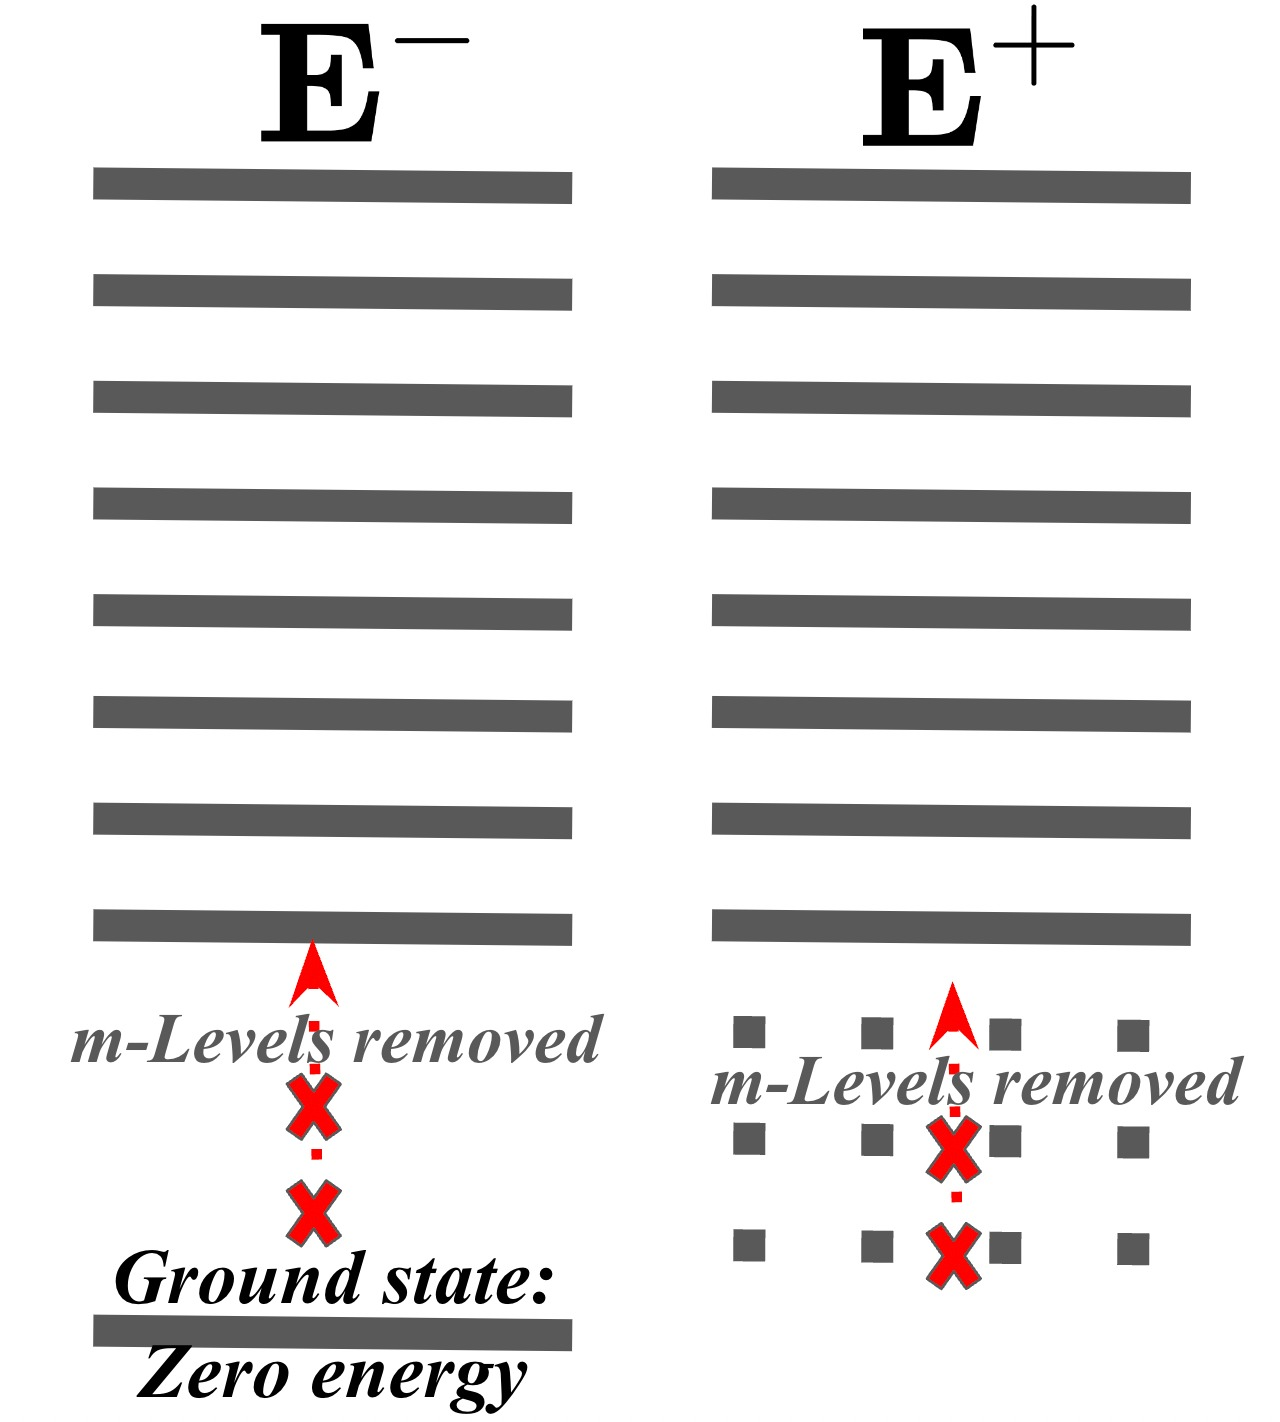
\includegraphics[height=0.55\textwidth,width=0.7\textwidth]{IMG/REHO-spectra.jpeg}
    \caption{Energy spectra of the partner Hamiltonian \(H^-\) and \(H^+\)}
\end{figure}
It should be noted that the eigenfunction of the hamiltonian \(H^-\) is a function of $X_m$ hermite polynomial with co-dimension $m$ and is orthogonal and complete with respect to $\frac{e^{-(\alpha x)^2}}{\mathcal{H}_m(\alpha x)^2}$. This $X_m$ hermite polynomial has missing degree upto $m$, that is, $X_6$ has $1, 2, 3, 4, 5$ and $6$ missing degrees. Similarly, $X_m$ has $1$ to $m$ missing degrees.




%------------Body-Ends--------------------
%\bibliography{ref.bib}
%\bibliographystyle{IEEEtran}
\end{document}
